\documentclass[10pt,a4paper,landscape]{article}
\usepackage{multicol}
\usepackage{calc}
\usepackage{ifthen}
\usepackage[landscape]{geometry}
\usepackage{amsmath,amsthm,amsfonts,amssymb}
\usepackage{color,graphicx}
\usepackage{hyperref}
\usepackage{listings}
\usepackage{underscore}
\usepackage{todonotes}

% Cheatsheet style
% Cheatsheet style

% This sets page margins to .5 inch if using letter paper, and to 1cm
% if using A4 paper. (This probably isn't strictly necessary.)
% If using another size paper, use default 1cm margins.
\ifthenelse{\lengthtest{\paperwidth = 11in}}
  % Then
  { \geometry{top=.5in,left=.5in,right=.5in,bottom=.5in} }
  % Else
  { \ifthenelse{\lengthtest{\paperwidth = 297mm}}
    {\geometry{top=1cm,left=1cm,right=1cm,bottom=1cm} }
    {\geometry{top=1cm,left=1cm,right=1cm,bottom=1cm} }
  }

% Turn off header and footer
\pagestyle{empty}

% Redefine section commands to use less space
\makeatletter
\renewcommand{\section}{\@startsection{section}{1}{0mm}%
                                {-1ex plus -.5ex minus -.2ex}%
                                {0.5ex plus .2ex}%x
                                {\color{darkred}\normalfont\large\bfseries}}
\renewcommand{\subsection}{\@startsection{subsection}{2}{0mm}%
                                {-1explus -.5ex minus -.2ex}%
                                {0.5ex plus .2ex}%
                                {\color{darkdarkred}\normalfont\normalsize\bfseries}}
\renewcommand{\subsubsection}{\@startsection{subsubsection}{3}{0mm}%
                                {-1ex plus -.5ex minus -.2ex}%
                                {1ex plus .2ex}%
                                {\normalfont\small\bfseries}}
\makeatother

% Define BibTeX command
\def\BibTeX{{\rm B\kern-.05em{\sc i\kern-.025em b}\kern-.08em
    T\kern-.1667em\lower.7ex\hbox{E}\kern-.125emX}}

% Don't print section numbers
\setcounter{secnumdepth}{0}

\setlength{\parindent}{0pt}
\setlength{\parskip}{0pt plus 0.5ex}

% Setting colors
\definecolor{lightgray}{rgb}{0.7,0.7,0.7}
\definecolor{lightergray}{rgb}{0.9,0.9,0.9}
\definecolor{darkblue}{rgb}{0.4,0.4,1}
\definecolor{darkred}{rgb}{0.9,0.2,0.2}
\definecolor{darkdarkred}{rgb}{0.6,0.0,0.0}
\definecolor{lightred}{rgb}{1,0.6,0.6}
\definecolor{lightgreen}{rgb}{0.6,1,0.6}
\definecolor{lightblue}{rgb}{0.6,0.8,1}
\definecolor{darkgreen}{rgb}{0.4,1,0.4}

% Set code listing style
\lstset {
    backgroundcolor=\color{lightgray},
    basicstyle=\ttfamily\scriptsize,
    breaklines=true,
}

\lstdefinestyle{bb}{
    backgroundcolor=\color{lightergray},
    frame=L,
    xleftmargin=\parindent,
}

% Set hyperlink style
\hypersetup{hidelinks}

% Enable figures
\newenvironment{colfig}
  {\par\medskip\noindent\minipage{\linewidth}}
  {\endminipage\par\medskip}

% Enable arg min/max math operators
\DeclareMathOperator*{\argmin}{arg\,min}
\DeclareMathOperator*{\argmax}{arg\,max}


% Shorthand for \bf
\providecommand{\bf}[1]{\ensuremath{\bf{#1}}}

\pdfinfo{
  /Title (Machine Learning Cheat Sheet)
  /Creator (TeX)
  /Producer (pdfTeX 1.40.0)
  /Author (Dennis Meier)
  /Subject (Machine Learning cheatsheet)
  /Keywords (machinelearning, ml, bayes, regression, classification)
}

% -----------------------------------------------------------------------

\begin{document}
\title{Machine Learning Cheat Sheet}

\raggedright
\footnotesize
\sffamily
\begin{multicols*}{4}

% multicol parameters
% These lengths are set only within the two main columns
%\setlength{\columnseprule}{0.25pt}
\setlength{\premulticols}{1pt}
\setlength{\postmulticols}{1pt}
\setlength{\multicolsep}{1pt}
\setlength{\columnsep}{2pt}

\begin{center}
  \Large{\underline{Machine Learning Cheat Sheet}}
\end{center}

% ----------
\section{Regression}
  $\mathcal{D}$ is a set of Training examples, the n-th Training Example ($n = 1,2, ..., N$), of this set is: $\bf{x}_n = \begin{bmatrix} x_{n1} \\ x_{n2} \\ ... \\ x_{nD} \end{bmatrix} $

  The goal is to predict a $\hat{y}$ given a $\bf{x}$.

  Simple linear regression: $y_n \approx \beta_0 + \beta_1 x_{n1}$

  Multiple linear regression: $y_n \approx f(\bf{x}_n) := \beta_0 + \beta_1 x_{n1} + \beta_2 x_{n2} + ... + \beta_D x_{nD}$

  \subsection{Linear basis function model}
  $y_n = \beta_0 + \sum_{i=1}^{M} \beta_i \phi_i(\bf{x_n}) =  \bf{\tilde\phi^T}(\bf{x}^T_n) \boldsymbol\beta$.
  The optimal $\beta$ is given by $\beta = ( \tilde{\Phi}^T \tilde{\Phi})^{-1} \tilde{\Phi}^T y$ where $\tilde{\Phi}$ is a matrix with N rows and the n-th row is $[1, \phi_1(x_n)^T,  ...,  \phi_M(x_n)^T]$.

  Ridge regression: $\beta_{ridge} = ( \tilde{\boldsymbol \Phi}^T \tilde{\boldsymbol\Phi} + \lambda \boldsymbol I)^{-1} \tilde{\boldsymbol\Phi}^T \boldsymbol y$

  \subsection{Cost functions}
  \begin{colfig}
    \centering
    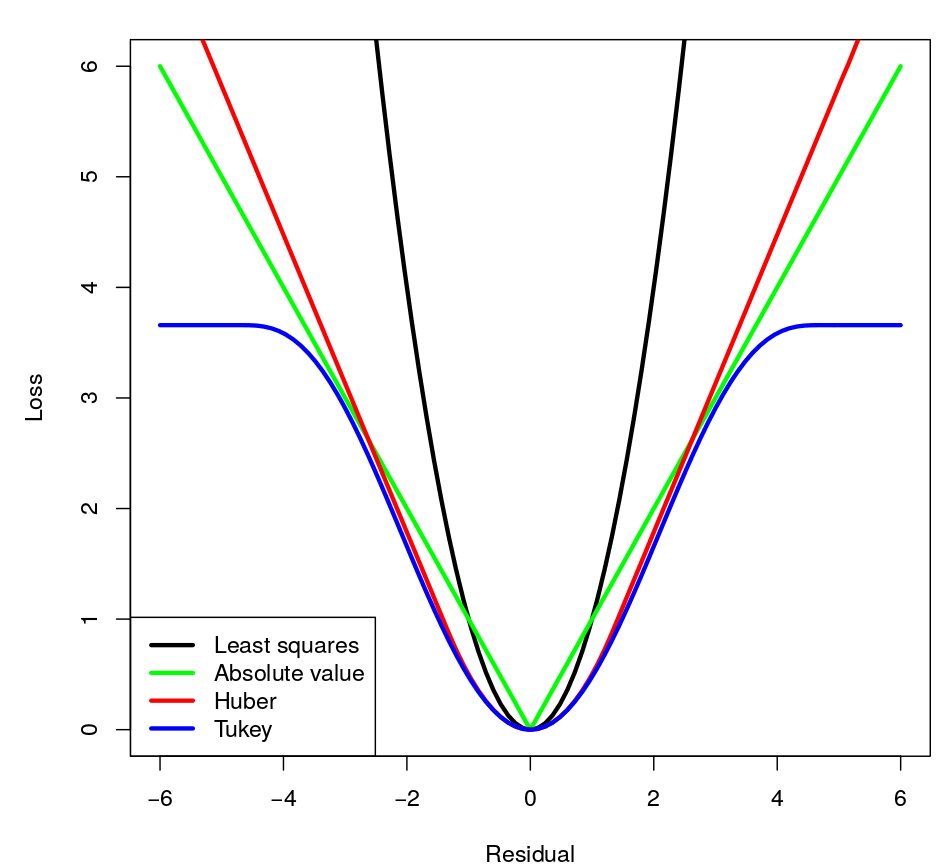
\includegraphics[width=\linewidth]{images/error-functions.png}
  \end{colfig}

  Cost function / Loss: $\mathcal{L}(\boldsymbol\beta) = \mathcal{L}(\mathcal{D},\boldsymbol\beta)$

  Mean square error (MSE): $\frac{1}{2N} \sum_{n=1}^{N}\left[y_n-f(\bf{x}_i) \right]^2$

  Mean absolute error (MAE): $\frac{1}{2N} \sum_{n=1}^{N}\left | y_n-f(\bf{x}_i) \right |$

  Huber loss: $\mathcal{L}_\delta (a) = \begin{cases}
   \frac{1}{2}{a^2}                   & \text{for } |a| \le \delta, \\
   \delta (|a| - \frac{1}{2}\delta ), & \text{otherwise.}
  \end{cases}$

  Root mean square error (RMSE): $\sqrt{2 * \text{MSE}}$

  Epsilon insensitive (used for SVMs):
  $\mathcal{L}_{\epsilon}(y, \hat{y}) = \begin{cases}
   0                   & \text{if } |y - \hat y| \le \epsilon, \\
   |y - \hat y| - \epsilon, & \text{otherwise.}
  \end{cases}$

% ----------
\section{Grid Search}
  Complexity: $\mathcal{O}(M^D N D)$, where $M$ is the number of grids in one dimension.

% ----------
\section{Gradient Descent}
  General rule: $\boldsymbol\beta^{(k+1)} = \boldsymbol\beta^{(k)} - \alpha \frac{\partial \mathcal{L}(\boldsymbol\beta^{(k)})}{\partial \boldsymbol\beta}$

  Complexity: $\mathcal{O}(I N D)$ where $I$ is the number of iterations we take.

  Big questions are how to get a good $\alpha$.

  The gradient for MSE comes out as:
  $\frac{\partial \mathcal{L}}{\partial \boldsymbol\beta} = - \frac{1}{N} \tilde{X}^T ( \boldsymbol y - \tilde{X} \boldsymbol\beta )$

% ----------
\section{Least squares}
  Complexity: $\mathcal{O}(ND^2 + D^3)$

  $\beta = ( \tilde{X}^T \tilde{X} )^{-1} \tilde{X}^T y$

% ----------
\section{Classification}
  Logistic Function $\sigma = \frac{exp(x)}{1+exp(x)}$

  Classification with linear regression: Use $y = 0$ as class $\mathcal{C_1}$
  and $y = 1$ as class $\mathcal{C_2}$ and then decide a newly estimated $y$ belongs
  to $\mathcal{C_1}$ if $y < 0.5$.

  \subsection{Logistic Regression}
  $\tilde{\bf{X}}^T [\sigma(\tilde{\bf{X}} \beta) - y] = 0$
  \todo[inline]{TODO: Generalized Linear model}

  \subsection{Error Functions}

  Root Mean square error (RMSE): $\sqrt{\frac{1}{N} \sum_{n=1}^{N}\left[y_n- \hat{p_n} \right]^2}$

  0-1 Loss: $ \frac{1}{N} \sum_{n=1}^{N} \delta(y_n, \hat{y_n})$

  logLoss: $- \frac{1}{N}  \sum_{n=1}^{N} y_n \log(\hat{p_n}) + (1-y_n) \log(1-\hat{p_n})$

% ----------
\section{Occam's Razor}
  It states that among competing hypotheses, the one with the fewest assumptions should be selected. Other, more complicated solutions may ultimately prove correct, but—in the absence of certainty—the fewer assumptions that are made, the better.

% ----------
\section{Bias-Variance Decomposition}
  \begin{colfig}
    \centering
    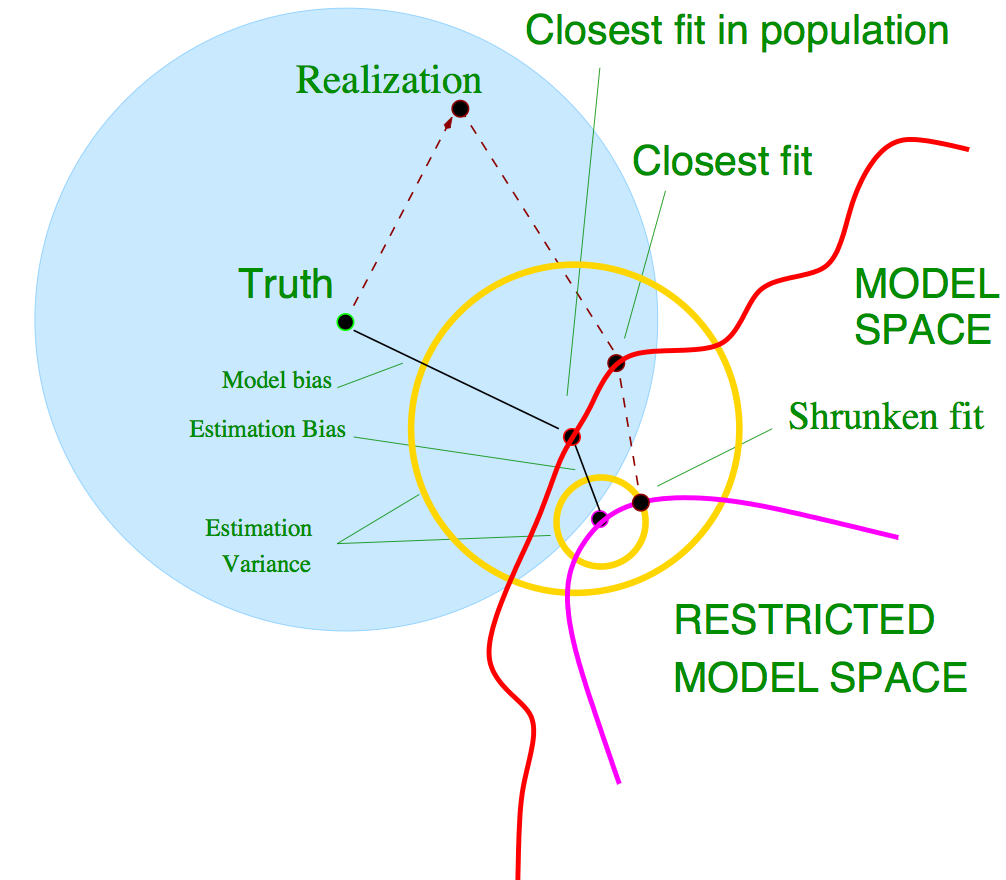
\includegraphics[width=\linewidth]{images/bias-variance.png}
  \end{colfig}

  \begin{tabular}{ l || c | c }
                            & bias & variance \\
    \hline
    regularization          & +    & - \\
    reduce model complexity & +    & - \\
    more data               & -    & \\
    \hline
  \end{tabular}

% ----------
\section{Maximum Likelihood}
  The Likelihood Function maps the model parameters to the probability distribution of $\bf{y}$:
  $\mathcal{L}_{lik}\colon \text{parameter space} \to [0;1]\quad  \bf{\beta} \mapsto p(\bf{y} \mid  \bf{\beta})$
  An underlying $p$ is assumed before. If the observed $y$ are IID, $p(\bf{y} \mid \beta) = \prod_n p(y_n \mid \beta)$.

  $\mathcal{L}_{lik}$ can be viewed as just another cost function. Maximum likelihood then simply choses the parameters $\bf{\beta}$ such that observed data is most likely. $\beta = \argmax_{\text{all} \beta} L(\beta)$

  Assuming different $p$ is basically what makes this so flexible. We can chose e.g.:

  \begin{tabular}{ l  l }
    \hline
    Gaussian $p$ & $\mathcal{L}_{lik} \widehat{=} \mathcal{L}_{MSE}$ \\
    Poisson $p$  & $\mathcal{L}_{lik} \widehat{=} \mathcal{L}_{MAE}$ \\
    \hline
  \end{tabular}

% ----------
\section{Bayesian methods}
  Bayes rule: $p(A, B) = p(A|B) p(B) = p(B|A) p(A)$

  The \textbf{prior} $p(\bf{f}|\bf{X})$ encodes our prior belief about the ``true'' model $\bf{f}$. The \textbf{likelihood} $p(\bf{y}|\bf{f})$ measures the probability of our (possibly noisy) observations given the prior.

  Least-squares tries to find model parameters $\bf{\beta}$ which maximize the likelihood. Ridge regression maximizes the \textbf{posterior} $p(\bf{\beta}|\bf{y})$

% ----------
\section{Kernel}
  Basically, Kernels are a mean to measure distance, or ``similarity'' of two vectors. We define:

  $(\bf{K})_{i,j} = \kappa(\bf{x_i}, \bf{x_j}) = \vec \phi(\bf{x_i})^T \vec \phi(\bf{x_j})$.

  The $\phi$ are not that important in the end, because we only use the Kernel as is. Sometimes it's even impossible to write them down explicitly.

  \begin{tabular}{ l | l }
    \hline
    Linear     & $\kappa(\bf{x_i}, \bf{x_j}) = \bf{x_i}^T \bf{x_j}$ \\
    \hline
    Polynomial & $\kappa(\bf{x_i}, \bf{x_j}) = (\bf{x_i}^T \bf{x_j} + c)^d$ \\
    \hline
    RBF        & $\kappa(\bf{x_i}, \bf{x_j}) = \exp\left(-\frac{||\bf{x_i} - \bf{x_j}||^2}{2\sigma^2}\right)$ \\
    \hline
  \end{tabular}

% ----------
\section{Support Vector Machines}
  Search for the hyperplane separating the data such that the gap is biggest.
  It minimizes the following cost function:

  $\mathcal{L}_{SVM} (\bf{\beta})= \sum_{n=1}^N [1 - y_n \tilde\phi_n \beta]_{+} + \frac{\lambda}{2} \sum_{j=1}^M \beta_j^2$

  This is convex but not differentiable.

% ----------
\section{Graphical Models}
  Bayes Net: Directed acyclic graph

  Belief propagation: graph between the observations and the variables is a bi-partite graph.

% ---------- Footer
\hrule
\tiny
Rendered \today. Written by Dennis Meier.
\copyright Dennis Meier. This work is licensed under the Creative Commons Attribution-ShareAlike 3.0 Unported License.
To view a copy of this license, visit http://creativecommons.org/licenses/by-sa/3.0/ or
send a letter to Creative Commons, 444 Castro Street, Suite 900, Mountain View, California, 94041, USA.

\includegraphics{images/by-sa.png}

\end{multicols*}
\end{document}
